\documentclass[aspectratio=169]{../latex_main/tntbeamer}  % you can pass all options of the beamer class, e.g., 'handout' or 'aspectratio=43'
\usepackage{dsfont}
\usepackage{bm}
\usepackage[english]{babel}
\usepackage[T1]{fontenc}
%\usepackage[utf8]{inputenc}
\usepackage{graphicx}
\graphicspath{ {./figures/} }
\usepackage{algorithm}
\usepackage[ruled,vlined,algo2e,linesnumbered]{algorithm2e}
\usepackage{hyperref}
\usepackage{booktabs}
\usepackage{mathtools}

\usepackage{amsmath,amssymb}

\DeclareMathOperator*{\argmax}{arg\,max}
\DeclareMathOperator*{\argmin}{arg\,min}

\usepackage{amsbsy}
\newcommand{\vect}[1]{\bm{#1}}
%\newcommand{\vect}[1]{\boldsymbol{#1}}

\usepackage{pgfplots}
\pgfplotsset{compat=1.16}
\usepackage{tikz}
\usetikzlibrary{trees} 
\usetikzlibrary{shapes.geometric}
\usetikzlibrary{positioning,shapes,shadows,arrows,calc,mindmap}
\usetikzlibrary{positioning,fadings,through}
\usetikzlibrary{decorations.pathreplacing}
\usetikzlibrary{intersections}
\pgfdeclarelayer{background}
\pgfdeclarelayer{foreground}
\pgfsetlayers{background,main,foreground}
\tikzstyle{activity}=[rectangle, draw=black, rounded corners, text centered, text width=8em]
\tikzstyle{data}=[rectangle, draw=black, text centered, text width=8em]
\tikzstyle{myarrow}=[->, thick, draw=black]

% Define the layers to draw the diagram
\pgfdeclarelayer{background}
\pgfdeclarelayer{foreground}
\pgfsetlayers{background,main,foreground}

% Requires XeLaTeX or LuaLaTeX
%\usepackage{unicode-math}

\usepackage{fontspec}
%\setsansfont{Arial}
\setsansfont{RotisSansSerifStd}[ 
Path=../latex_main/fonts/,
Extension = .otf,
UprightFont = *-Regular,  % or *-Light
BoldFont = *-ExtraBold,  % or *-Bold
ItalicFont = *-Italic
]
\setmonofont{Cascadia Mono}[
Scale=0.8
]

% scale factor adapted; mathrm font added (Benjamin Spitschan @TNT, 2021-06-01)
%\setmathfont[Scale=1.05]{Libertinus Math}
%\setmathrm[Scale=1.05]{Libertinus Math}

% other available math fonts are (not exhaustive)
% Latin Modern Math
% XITS Math
% Libertinus Math
% Asana Math
% Fira Math
% TeX Gyre Pagella Math
% TeX Gyre Bonum Math
% TeX Gyre Schola Math
% TeX Gyre Termes Math

% Literature References
\newcommand{\lit}[2]{\href{#2}{\footnotesize\color{black!60}[#1]}}

%%% Beamer Customization
%----------------------------------------------------------------------
% (Don't) Show sections in frame header. Options: 'sections', 'sections light', empty
\setbeamertemplate{headline}{empty}

% Add header logo for normal frames
\setheaderimage{
	% 
\includegraphics[height=\logoheight]{figures/TNT_darkv4.pdf}
	
\includegraphics[height=\logoheight]{../latex_main/figures/luh_logo_rgb_0_80_155.pdf}
	% 
\includegraphics[height=\logoheight]{figures/logo_tntluh.pdf}
}

% Header logo for title page
\settitleheaderimage{
	% 
\includegraphics[height=\logoheight]{figures/TNT_darkv4.pdf}
	
\includegraphics[height=\logoheight]{../latex_main/figures/luh_logo_rgb_0_80_155.pdf}
	% 
\includegraphics[height=\logoheight]{figures/logo_tntluh.pdf}
}

% Title page: tntdefault 
\setbeamertemplate{title page}[tntdefault]  % or luhstyle
% Add optional title image here
%\addtitlepageimagedefault{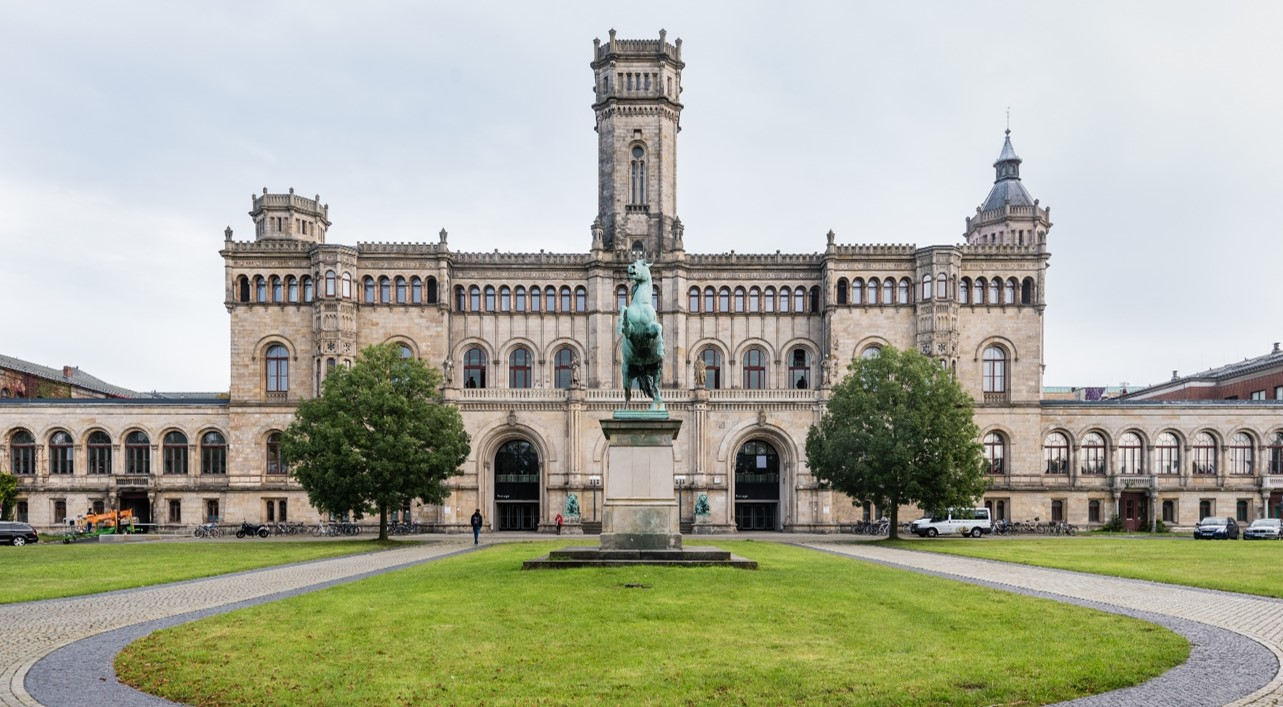
\includegraphics[width=0.65\textwidth]{figures/luh_default_presentation_title_image.jpg}}

% Title page: luhstyle
% \setbeamertemplate{title page}[luhstyle]
% % Add optional title image here
% \addtitlepageimage{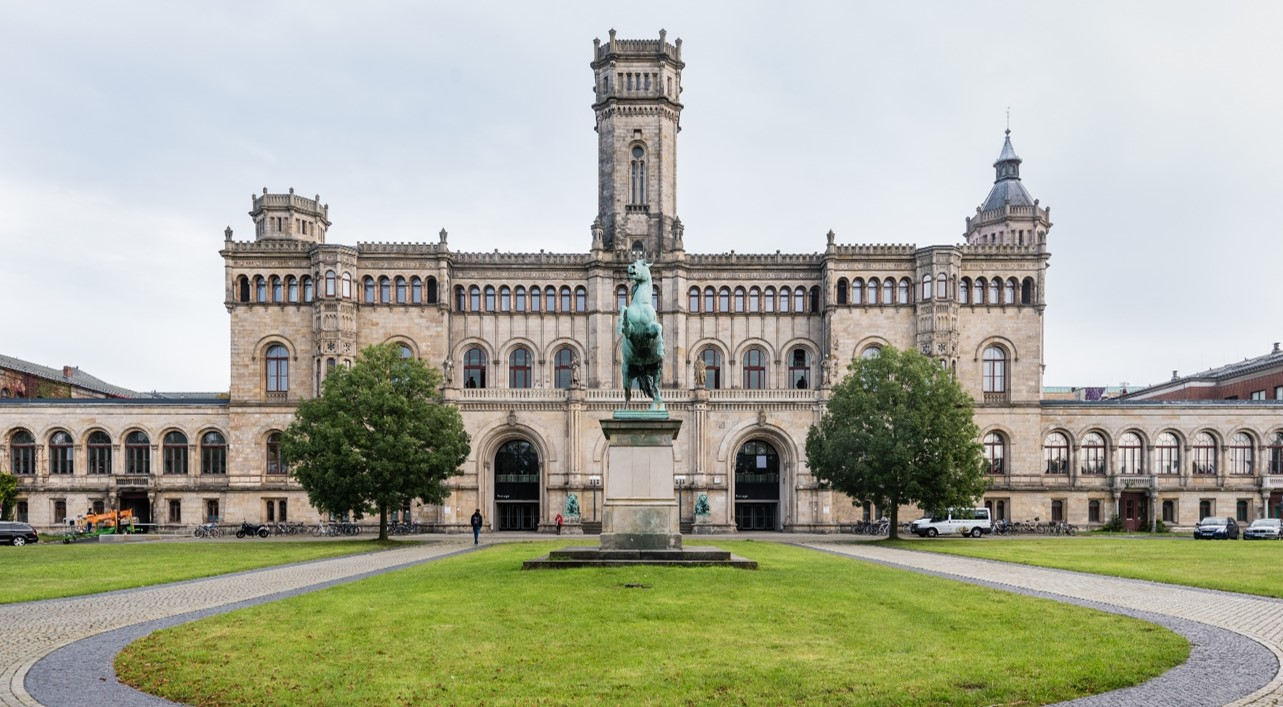
\includegraphics[width=0.75\textwidth]{figures/luh_default_presentation_title_image.jpg}}

\author[Abedjan \& Lindauer]{Ziawasch Abedjan \& Marius Lindauer\\[1em]
	
\includegraphics[height=\logoheight]{../latex_main/figures/luh_logo_rgb_0_80_155.pdf}\qquad
	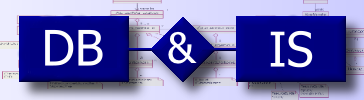
\includegraphics[height=\logoheight]{../latex_main/figures/DBIS_Kurzlogo.png}\qquad

\includegraphics[height=\logoheight]{../latex_main/figures/TNT_darkv4}\qquad

\includegraphics[height=\logoheight]{../latex_main/figures/L3S.jpg}	}
\date{Summer Term 2022; \hspace{0.5em} {
\includegraphics[height=1.5em]{../latex_main/figures/Cc-by-nc-sa_icon.svg.png}}; based on \href{https://ds100.org/fa21/}{[DS100]}
}


%%% Custom Packages
%----------------------------------------------------------------------
% Create dummy content
\usepackage{blindtext}

% Adds a frame with the current page layout. Just call \layout inside of a frame.
\usepackage{layout}


%%% Macros
%\renewcommand{\vec}[1]{\mathbf{#1}}
% \usepackage{bm}
%\let\vecb\bm

\title[Introduction]{DS: Dimension Reduction}
\subtitle{t-distributed Stochastic Neighbor Embedding t-SNE}

\graphicspath{ {./figure/} }
%\institute{}


\begin{document}
	
	\maketitle
	\begin{frame}[c]{Motivation}
	    
	    \begin{itemize}
	        \item PCA focuses on the global trend of the data\\
	        but does not ensure that the neighborhood is preserved
	        \pause
	        \item One can argue that the global trend might be important as long as similar points are still similar in the low-dimensional space
	        \begin{itemize}
	            \item Later on, a good model should predict similar $y$ for similar points
	            \item[$\leadsto$] Also important from a fairness point of view
	        \end{itemize}
	        \pause
	        \item Similar to MDS, but modelled with probabilities,
	        \begin{itemize}
	            \item chance of correct neighborhood should increase with similarity in the orignal space
	            \item allows for efficient computing of the low-dimensional representation
	        \end{itemize}
	    \end{itemize}
	    
	\end{frame}
	
	\begin{frame}[c]{Probabilistic Setting}
	    
	    $$ p_{j\mid i } = \frac{\exp(- || x_i - x_j||^2 / 2\sigma_i^2)}{\sum_{k\neq i}  \exp(- || x_i - x_k||^2 / 2\sigma_i^2) } $$
	    
	    \begin{itemize}
	        \item Being a neighbor is proportional to the probability density under a Gaussian around $x_i$
	        \item $p_{i\mid i} = 0$ and $\sum_j p_{j\mid i} = 1$
	        \item $\sigma_i$ is estimated s.t. it relates to a predefined perplexity
	        \begin{itemize}
	            \item Perplexity: How good can a probability distribution predict a sample
	            \item[$\leadsto$] Smaller $\sigma_i$ in denser parts of the space
	        \end{itemize}
	    \end{itemize}
	    
	    \pause
	    
	    $$ p_{ij} = \frac{p_{j\mid i} + p_{i\mid j}}{2N}$$
	    
	\end{frame}
	
	
	\begin{frame}[c]{Projection into the Low-Dimensional Space}
	    
	    Similarity measure in the low-dimensional space:
	    
	    $$q_{ij} = \frac{ (1 + ||x'_i - x'_j ||^2) ^{-1}}{\sum_k \sum_{l\neq k} (1+ ||x'_k - x'_y||^2)^{-1}} $$
	    
	    \begin{itemize}
	        \item heavy-tailed Student t-distribution
	        \item[$\leadsto$] allows to model dissimilar points being far apart in the low-dimensional space
	        \begin{itemize}
	            \item Hard to achieve with a Gaussian distribution because it is not heavy-tailed
	        \end{itemize}
	    \end{itemize}
	    
	    \pause
	    
	    Minimize Kullback-Leibler divergence between both distributions:
	    
	    $$KL(P \parallel  Q) = \sum_{i \neq j} p_{ij} \log \frac{p_{ij}}{q_{ij}}$$
	    
	    \begin{itemize}
	        \item Can be efficiently done via Gradient Descent
	    \end{itemize}
	    
	\end{frame}
	
	
	\begin{frame}{Example}
	
	\begin{columns}
	
	\begin{column}{0.5\textwidth}
	
	  \centering
	 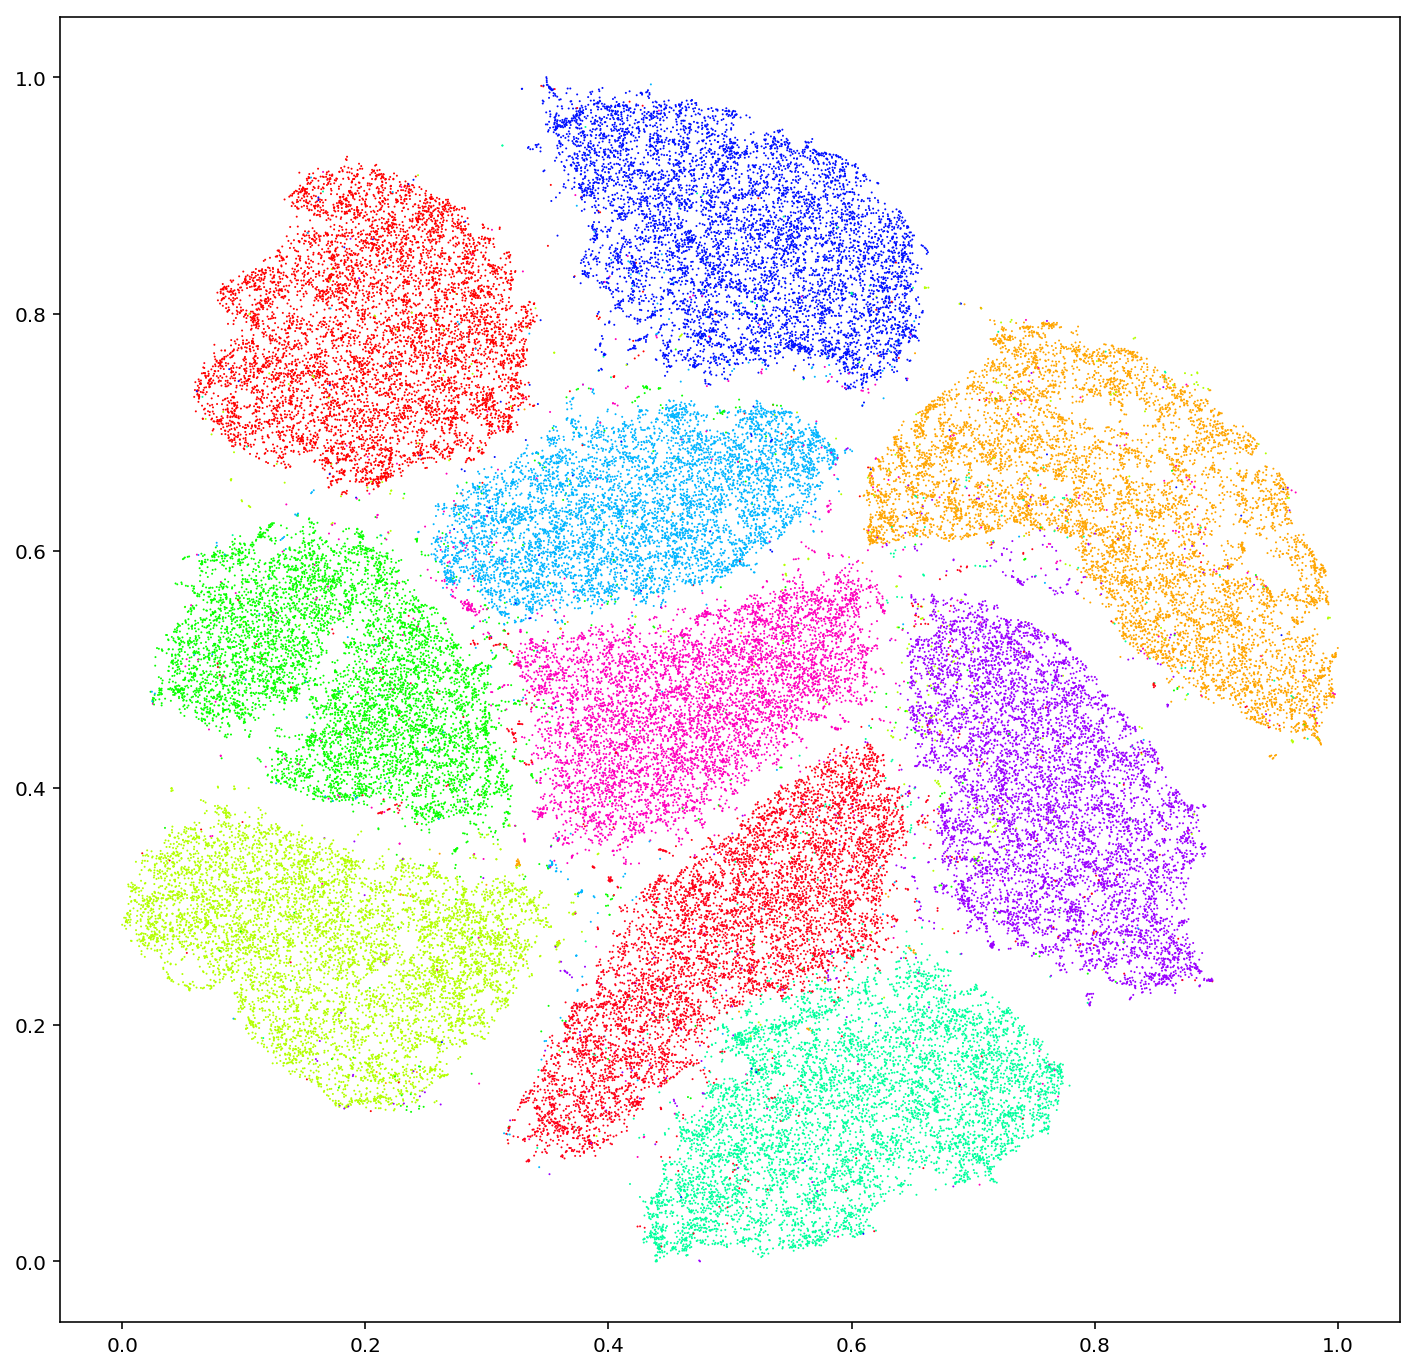
\includegraphics[width=.7\textwidth]{T-SNE_Embedding_of_MNIST.png}\\ 
	 \small Source: \href{https://commons.wikimedia.org/wiki/File:T-SNE_Embedding_of_MNIST.png}{[Kyle McDonald Wikipedia]}
	
	\end{column}
		
	\begin{column}{0.5\textwidth}

    \begin{itemize}
        \item Often you see clusters in these plots, referring to different classes
        \item You could use a cluster algorithm if you don't have $y$ values
    \end{itemize}	

	\end{column}
	
	\end{columns}
	    
	\end{frame}
	
	
	\begin{frame}{Traits}
	    
	    Advantages:
	    \begin{itemize}
	        \item Preserves well the local neighborhood
	        \item Can be efficiently computed
	        \item Works very well for image data
	    \end{itemize}
	    
	    \pause
	    
	    Disadvantages:
	    \begin{itemize}
	        \item Can suffer from curse of dimensionality in too high-dimensional spaces
	        \item If t-SNE is not working well, models depending on Euclidean distances might also fail
	        \begin{itemize}
	            \item \textbf{Could} also be an indicator that your input feature space lacks information
	        \end{itemize}
	        \item Comes with perplexity threshold as hyperparameter that can substantially change your low-dimensional space
	        \item global structure (e.g., cluster size or distance between clusters) have no meaning
	        \item[$\leadsto$] Please read before using \url{https://distill.pub/2016/misread-tsne/}
	    \end{itemize}
	    
	\end{frame}
	
\end{document}